% Foliensatz: "AFu-Kurs nach DJ4UF" von DK0TU, Amateurfunkgruppe der TU Berlin
% Lizenz: CC BY-NC-SA 3.0 de (http://creativecommons.org/licenses/by-nc-sa/3.0/de/)
% Autoren: Felix Baum DB4UM <baum@campus.tu-berlin.de>

\documentclass[aspectratio=169]{beamer}

\usepackage[ngerman]{babel} % deutsche Worttrennung etc.
\usepackage[utf8]{inputenc} % UTF8 Text

\usepackage[super, comma, numbers, square, sort]{natbib}

\usepackage{hyperref}       % Hyperref Package für bessere Referenzen (todo)
\hypersetup{
	colorlinks=false,       %   false: boxed links; true: colored links
    %linkcolor=white,       %   color of internal links (change box color with linkbordercolor)
    citecolor=red,          %   color of links to bibliography
    filecolor=white,        %   color of file links
    urlcolor=blue           %   color of external links
}

\usepackage{multirow}
\usepackage{wasysym}  % Math Symbols like \permil
%\usepackage{colortbl}
%\usepackage{subscript}
%\usepackage{caption}
%\usepackage{setspace}
%\usepackage{xcolor}        % benutze CodeListe

% Footnote
%\usepackage{hanging}
%
%\setbeamertemplate{footnote}{%
%  \hangpara{2em}{1}%
%  \makebox[2em][l]{\insertfootnotemark}\footnotesize\insertfootnotetext\par%
%}


%\usepackage{pgf}
%\usepackage{tikz}
%\usetikzlibrary{arrows,automata}
%\usetikzlibrary{positioning}
%
%\tikzset{
%    state/.style={
%           rectangle,
%           rounded corners,
%           draw=black, very thick,
%           minimum height=2em,
%           minimum width=2pt,
%           inner sep=2pt,
%           text centered,
%           },
%}

%\usepackage{listings}
%\lstset{basicstyle=\small, numberstyle=\tiny, extendedchars=true, numbers=left, numbersep=5pt}
%\lstset{showtabs=false, showspaces=false, showstringspaces=false}
%%\lstset{backgroundcolor=\color{white!75!lightgray}, , frame=single}
%%\lstset{backgroundcolor=\color{white}}
%%\lstset{backgroundcolor=none}
%\lstset{keywordstyle=\color{blue!50!gray},  identifierstyle=\color{black}}
%\lstset{commentstyle=\color{green!50!gray}, stringstyle=\color{red!50!gray}}
%\lstset{language=C, fontadjust=true, tabsize=2, breaklines=true}
%\lstset{backgroundcolor=\color{white!75!lightgray}, caption=\lstname, frame=single}
%\lstset{emphstyle=\color{black}\fbox}
%
%% Keine "Listing:"-Caption
%\captionsetup{labelformat=empty,labelsep=none}
%
%% für mathematische Umgebungen
%\usepackage{amsmath,amsfonts,amssymb}
%
%\lstdefinestyle{Bash}{
%language=Bash,
%frame=single,
%rulecolor=\color{black},
%backgroundcolor=\color{gray!50},
%keywordstyle=\color{black},
%identifierstyle=,
%commentstyle=\color{black},
%stringstyle=\color{magenta!65!white},
%showstringspaces=false,
%basicstyle=\footnotesize\ttfamily\color{black},
%numbers=none,
%breaklines=true,
%captionpos=b
%}

%\usepackage{listings}
%
%\lstdefinestyle{basic}{
%    captionpos=t,%
%    basicstyle=\footnotesize\ttfamily,%
%    numberstyle=\tiny,%
%    numbers=left,%
%    stepnumber=1,%
%    frame=single,%
%    showspaces=false,%
%    showstringspaces=false,%
%    showtabs=false,%
%    %
%    keywordstyle=\color{blue},%
%    identifierstyle=,%
%    commentstyle=\color{gray},%
%    stringstyle=\color{magenta}%
%}



% fließende Boxen haben keinen Abstand
%\fboxsep0mm

% inkludiere Creative Commons Helper
%%%%%%%%%%%%%%%%%%%%%%%%%%%%%%%%%%%%%%%%%%%%%%%%%%%%%%%%%%%%%%%%
%% ccBeamer 0.1, 2007-07-02                                   %%
%% Written by Sebastian Pipping <webmaster@hartwork.org>      %%
%% ---------------------------------------------------------- %%
%% Licensed under Creative Commons Attribution-ShareAlike 3.0 %%
%% http://creativecommons.org/licenses/by-sa/3.0/             %%
%%%%%%%%%%%%%%%%%%%%%%%%%%%%%%%%%%%%%%%%%%%%%%%%%%%%%%%%%%%%%%%%


%% Images
\newcommand{\CcImageBy}[1]{%
	
\includegraphics[scale=#1]{texdata/creative_commons/cc_by_30.pdf}%
}
\newcommand{\CcImageCc}[1]{%
	
\includegraphics[scale=#1]{texdata/creative_commons/cc_cc_30.pdf}%
}
\newcommand{\CcImageDevNations}[1]{%
	
\includegraphics[scale=#1]{texdata/creative_commons/cc_dev_nations_30.pdf}%
}
\newcommand{\CcImageNc}[1]{%
	
\includegraphics[scale=#1]{texdata/creative_commons/cc_nc_30.pdf}%
}
\newcommand{\CcImageNd}[1]{%
	
\includegraphics[scale=#1]{texdata/creative_commons/cc_nd_30.pdf}%
}
\newcommand{\CcImagePd}[1]{%
	
\includegraphics[scale=#1]{texdata/creative_commons/cc_pd_30.pdf}%
}
\newcommand{\CcImageSa}[1]{%
	
\includegraphics[scale=#1]{texdata/creative_commons/cc_sa_30.pdf}%
}
\newcommand{\CcImageSampling}[1]{%
	
\includegraphics[scale=#1]{texdata/creative_commons/cc_sampling_30.pdf}%
}
\newcommand{\CcImageSamplingPlus}[1]{%
	
\includegraphics[scale=#1]{texdata/creative_commons/cc_sampling_plus_30.pdf}%
}


%% Groups
\newcommand{\CcGroupBy}[2]{% zoom, gap
	\CcImageCc{#1}\hspace*{#2}\CcImageBy{#1}%
}
\newcommand{\CcGroupByNc}[2]{% zoom, gap
	\CcImageCc{#1}\hspace*{#2}\CcImageBy{#1}\hspace*{#2}\CcImageNc{#1}%
}
\newcommand{\CcGroupByNcNd}[2]{% zoom, gap
	\CcImageCc{#1}\hspace*{#2}\CcImageBy{#1}\hspace*{#2}\CcImageNc{#1}\hspace*{#2}\CcImageNd{#1}%
}
\newcommand{\CcGroupByNcSa}[2]{% zoom, gap
	\CcImageCc{#1}\hspace*{#2}\CcImageBy{#1}\hspace*{#2}\CcImageNc{#1}\hspace*{#2}\CcImageSa{#1}%
}
\newcommand{\CcGroupByNd}[2]{% zoom, gap
	\CcImageCc{#1}\hspace*{#2}\CcImageBy{#1}\hspace*{#2}\CcImageNd{#1}%
}
\newcommand{\CcGroupBySa}[2]{% zoom, gap
	\CcImageCc{#1}\hspace*{#2}\CcImageBy{#1}\hspace*{#2}\CcImageSa{#1}%
}
\newcommand{\CcGroupDevNations}[2]{% zoom, gap
	\CcImageCc{#1}\hspace*{#2}\CcImageDevNations{#1}%
}
\newcommand{\CcGroupNcSampling}[2]{% zoom, gap
	\CcImageCc{#1}\hspace*{#2}\CcImageNc{#1}\hspace*{#2}\CcImageSampling{#1}%
}
\newcommand{\CcGroupPd}[1]{% zoom
	\CcImagePd{#1}%
}
\newcommand{\CcGroupSampling}[1]{% zoom
	\CcImageSampling{#1}%
}
\newcommand{\CcGroupSamplingPlus}[1]{% zoom
	\CcImageSamplingPlus{#1}%
}


%% Text
\newcommand{\CcLongnameBy}{Attribution}
\newcommand{\CcLongnameByNc}{Attribution-NonCommercial}
\newcommand{\CcLongnameByNcNd}{Attribution-NoDerivs}
\newcommand{\CcLongnameByNcSa}{Attribution-NonCommercial-ShareAlike}
\newcommand{\CcLongnameByNd}{Attribution-NoDerivs}
\newcommand{\CcLongnameBySa}{Attribution-ShareAlike}

\newcommand{\CcNote}[1]{% longname
	This work is licensed under the \textit{Creative Commons #1 3.0 License}.%
}


% generelles Thema auswählen
\usetheme{Goettingen} %Berlin spart ohne Sidebar allerdings angenehm Platz
% AnnArbor | Antibes | Bergen | Berkeley | Berlin | Boadilla | boxes | CambridgeUS | Copenhagen | Darmstadt | default | Dresden | Frankfurt | Goettingen | Hannover | Ilmenau | JuanLesPins | Luebeck | Madrid | Malmoe | Marburg | Montpellier | PaloAlto | Pittsburgh | Rochester | Singapore | Szeged | Warsaw

% Farben wählen
\usecolortheme{beetle}
% beaver | beetle | crane | default | dolphin | dove | fly | lily | orchid | rose | seagull | seahorse | sidebartab | structure | whale | wolverine

% Setze alle Farben auf Grau und Weiß
%\definecolor{craneorange}{RGB}{64,64,64}
%\definecolor{craneblue}{RGB}{255,255,255}

% Schriftart wählen
\usefonttheme{default}
% default | professionalfonts | serif | structurebold | structureitalicserif | structuresmallcapsserif

% Innere Themen(Kopf-, Fuß-, Sidebar usw)
%\useinnertheme{default}
\useinnertheme{circles}
% default | inmargin | rectangles | rounded | circles

% Äußere Themen (Anordnung der inneren, grenzen der Folien etc.)
\useoutertheme{infolines}
% default | infolines | miniframes | shadow | sidebar | smoothbars | smoothtree | split | tree

% Deaktiviere Navigations-Symbole ({} -> leer)
\setbeamertemplate{navigation symbols}{}
%\setbeamertemplate{navigation symbols}{\large \ifnum \insertframenumber <10 0\fi\insertframenumber/\inserttotalframenumber\vspace*{0.2ex}}

% Zeige ein Hintergrundbild
\setbeamertemplate{background canvas}{
        \hspace*{-2.0cm}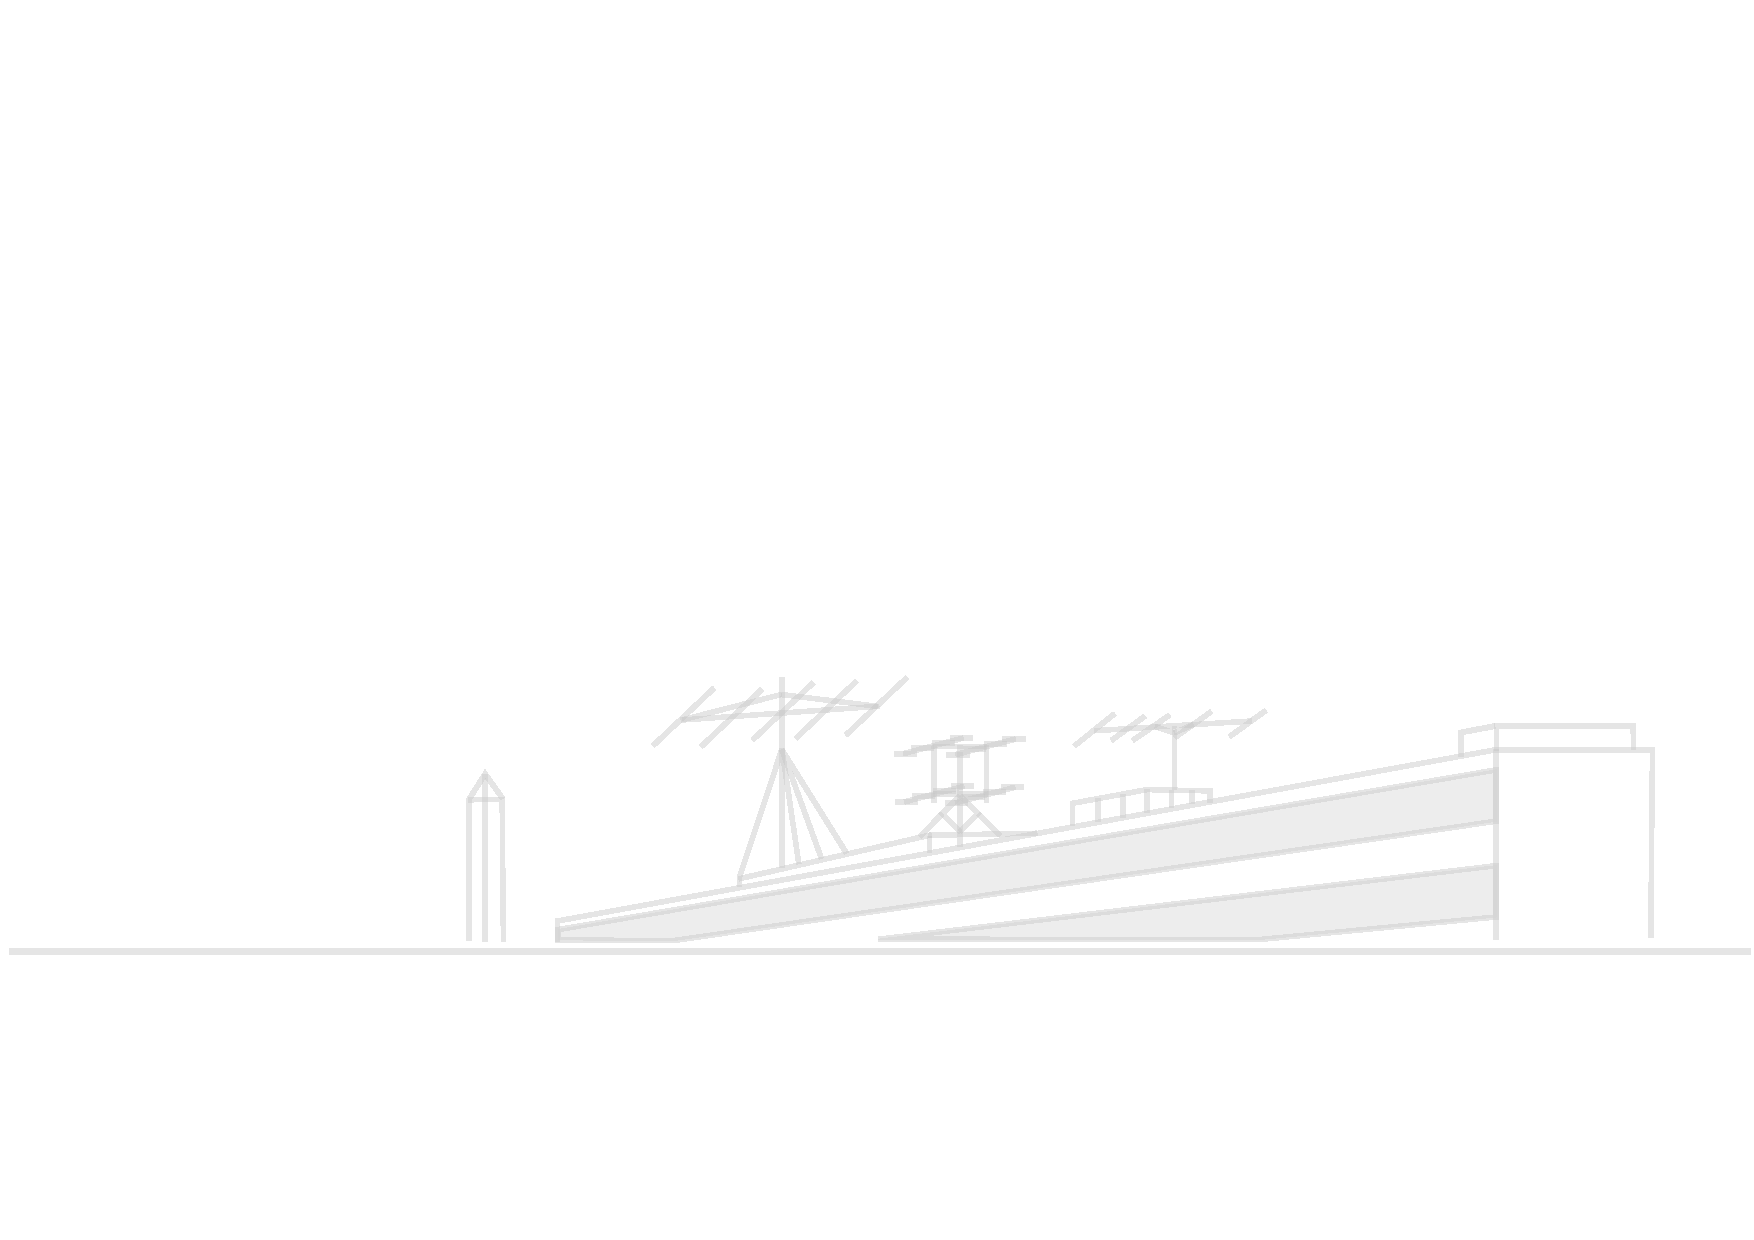
\includegraphics[width=17.8cm]{texdata/dk0tu_rooftop_background.pdf}
}

% Foliennummer einfügen
\setbeamertemplate{footline}[frame number]
%\setbeamertemplate{footline}{}

% Ändere das Zeichen vor jedem item
%\setbeamertemplate{itemize item}{\color{craneorange}$\blacktriangleright$}
%\setbeamertemplate{itemize subitem}{\color{craneorange}$\triangleright$}
%\setbeamertemplate{itemize subsubitem}{\color{craneorange}$\blacktriangleright$}

% Ändert die Blöcke 
\setbeamertemplate{blocks}[rounded][shadow=true]
% default | rounded [shadow=true|false]

%
% Eigene Kommandos
%

% Hack to get natbib and beamer working together. "The beamer user guide suggests
% that only the manual bibliography entry approach is supported"
% on some system it works out of the box, sometimes you need the hack :-(
% so check it --dl7bst
\ifdefined\newblock
    \relax
\else
    \newcommand{\newblock}{}
\fi

% \includedia command to generate png out of a dia file
% NEEDS installed dia and pdflatex option --shell-escape
\newcommand{\includedia}[1]{
    \immediate\write18{/usr/bin/dia #1.dia -e #1_diatmp.png -t png}
}

% RICHIG GROSSER FONT!
\newfont{\bigfont}{cmr10 at 144pt}
\newfont{\smallfont}{cmr10 at 8pt}

% Römische Ziffern
\makeatletter
\newcommand{\rmnum}[1]{\romannumeral #1}
\newcommand{\Rmnum}[1]{\expandafter\@slowromancap\romannumeral #1@}
\makeatother

% Schwarze Überschrift
%\setbeamercolor{frametitle}{fg=black}
%\setbeamercolor{title}{fg=black}

% Item- und Box-Farben
\definecolor{deepBlue}{HTML}{000066}
\setbeamercolor{itemize item}{fg=deepBlue}
\setbeamercolor{itemize subitem}{fg=deepBlue}
\setbeamercolor{description item}{fg=deepBlue}
\setbeamercolor{block title}{fg=deepBlue!100, bg=blue!15}
\setbeamercolor{block body}{fg=black, bg=blue!5}
\setbeamercolor{block title alerted}{fg=deepBlue, bg=red!75}
\setbeamercolor{block body alerted}{fg=black, bg=red!15}
\setbeamercolor*{block title example}{fg=blue!50, bg=blue!10}
\setbeamercolor*{block body example}{fg= blue, bg=blue!5}

%\setbeamercolor{section in head/foot}{parent=palette primary}
%\setbeamercolor{subsection in head/foot}{parent=palette secondary}
%\setbeamercolor{sidebar}{fg=darkblue,bg=yellow!90!orange}
%\setbeamercolor{title in sidebar}{fg=darkblue}
%\setbeamercolor{author in sidebar}{fg=darkblue}
%\setbeamercolor{section in sidebar}{fg=darkblue!10!black}
%\setbeamercolor{subsection in sidebar}{fg=darkblue!50!black}

% Titlepage Infos
\title{AFu-Kurs nach DJ4UF}
\author[DKØTU]{DKØTU\\ \footnotesize{Amateurfunkgruppe der TU Berlin}}
\institute[DKØTU]{\url{http://www.dk0tu.de} }

% PDF-Eigenschaften
\subject{DK0TU-Amateurfunkkurs nach DJ4UF}
\keywords{Amateurfunk Kurs HAM Radio Course CC-BY-NC-SA OpenSource TU Berlin DK0TU}

\subtitle{Technik A07: \\
           Oszillator und Hochfrequenzverstärker \\[2em]}
\date{Stand 17.5.2015}
 \begin{document}

\begin{frame}
    \titlepage
    \vfill
    \begin{center}
        \ccbyncsaeu\\
        {\tiny This work is licensed under the \em{Creative Commons Attribution-NonCommercial-ShareAlike 3.0 License}.}\\[0.5ex]
         \tiny Amateurfunkgruppe der Technische Universität Berlin (AfuTUB), DKØTU
         %\includegraphics[scale=0.5]{img/DK0TU_Logo.pdf}
    \end{center}
\end{frame}


\section*{Wiederholung}

\begin{frame}
    \frametitle{Verstärker Wiederholung}
    \begin{center}
    \large Um was für eine Transistorschaltung handelt es sich?
        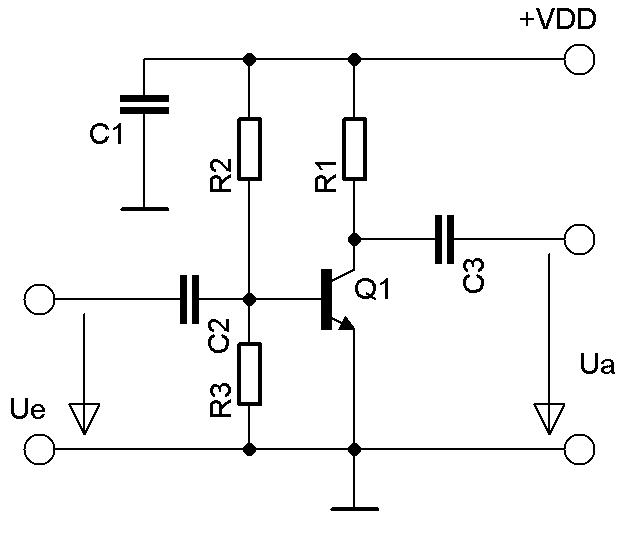
\includegraphics[width=0.7\textwidth]{a07/Transistor_Verstaerker_emetter.png}
	\end{center}
\end{frame}

\begin{frame}
    \frametitle{Verstärker Wiederholung}
    \begin{center}
    \large Emitterschaltung, da der Emitter auf dem gemeinsamen potential liegt.\\
    Phasendrehung von $180$ Grad
        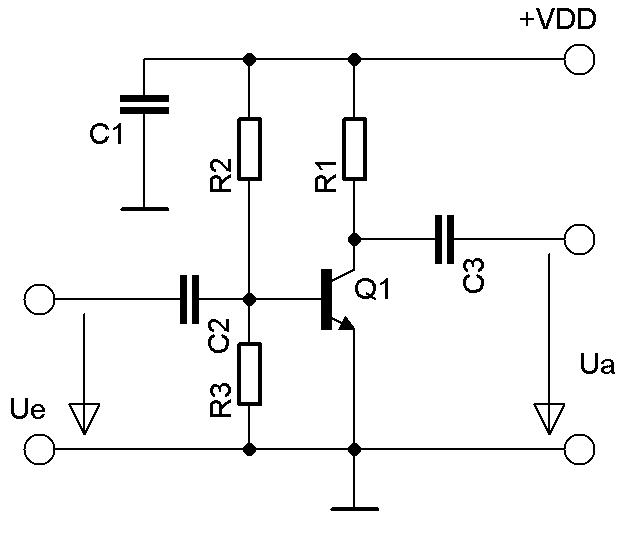
\includegraphics[width=0.5\textwidth]{a07/Transistor_Verstaerker_emetter.png}
	\end{center}
\end{frame}

\section*{Verstärkung vs Bandbreite}

\begin{frame}
    \frametitle{Verstärkungsbandbreiteprodukt}
    \begin{center}
        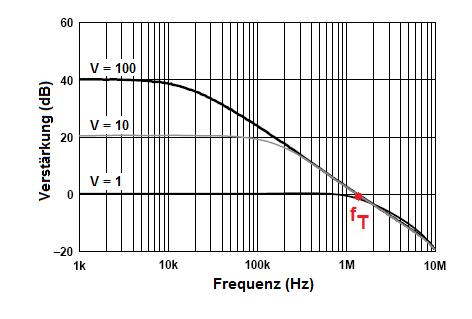
\includegraphics[width=0.7\textwidth]{a07/Closed_loop_gain.png}
        \tiny \hyperlink{refs}{\cite{wm}} \\[3em]
     	\large Aufgrund von Kapazitäten im Transistor geringer Welchselstromwiederstand und somit geringe Verstärkung
     \end{center}
\end{frame}

\begin{frame}
    \frametitle{Ersatzschaltbild Mosfet mit Kapazitäten}
    \begin{center}
        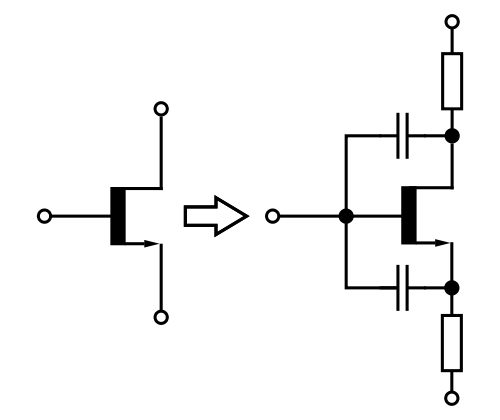
\includegraphics[width=0.7\textwidth]{a07/HF_Ersatzschaltbild.png}
        \tiny \hyperlink{refs}{\cite{wm}} \\[3em]
     	\large Probleme mit Kapazitäten im Mosfet (Gate und Drain/Source, wie Kapazitätsdioden)
     \end{center}
\end{frame}

\begin{frame}
    \frametitle{Breitband Verstärker}
    \begin{center}
        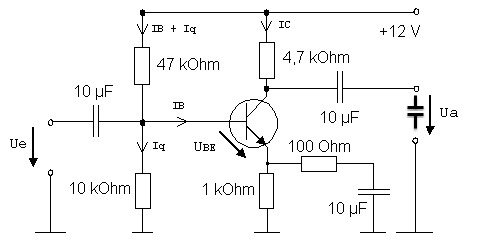
\includegraphics[width=0.7\textwidth]{a07/Breitbandverstarker.png}
        \tiny \hyperlink{refs}{\cite{wm}} \\[3em]
     	\large Ausgangslast bei HF auch kaum noch Impedanz
     \end{center}
\end{frame}

\begin{frame}
    \frametitle{Selektiver Verstärker}
    \begin{center}
        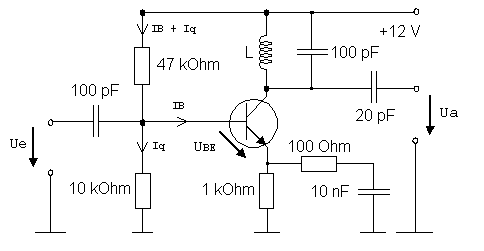
\includegraphics[width=0.7\textwidth]{a07/Selektiver_Verstarker.png}
        \tiny \hyperlink{refs}{\cite{wm}} \\[3em]
     	\large Ausgangslast Teil des Schwingkreises, somit bei Sperrfrequenz hoher Widerstand
     \end{center}
\end{frame}
  
\section*{Oszillator}

\begin{frame}
    \frametitle{Rückgekoppelte Systeme / Schwingbedingungen}
        \begin{center}
        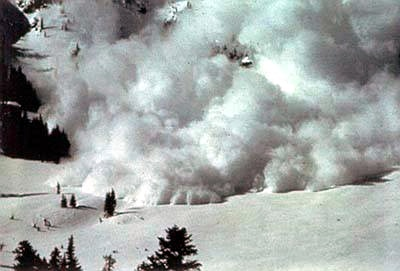
\includegraphics[width=1\textwidth]{a07/Lawine.jpg}
        \tiny \hyperlink{refs}{\cite{wm}} \\
     	\large Eine Mittkopplung des Schnees. Ein wenig Schnee beginnt und Reißt immer mehr mit
     \end{center}
\end{frame}

\begin{frame}
    \frametitle{Rückgekoppelte Systeme / Schwingbedingungen}
    \begin{center}
        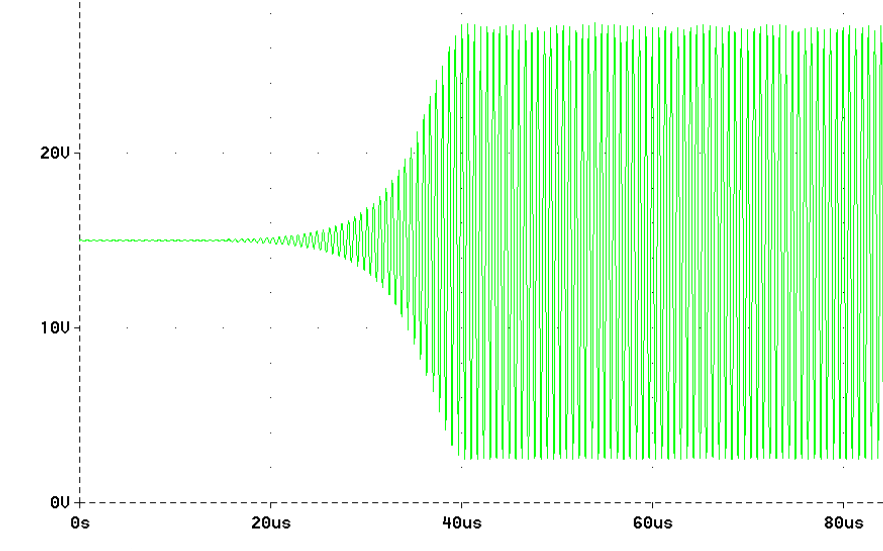
\includegraphics[width=1\textwidth]{a07/Oszillator_Anschwingen.png}
        \tiny \hyperlink{refs}{\cite{wm}} \\[3em]
     	\large Anschwingen eines Oszillators
     \end{center}
\end{frame}

\begin{frame}
    \frametitle{Rückgekoppelte Systeme / Schwingbedingungen}
        \begin{center}
        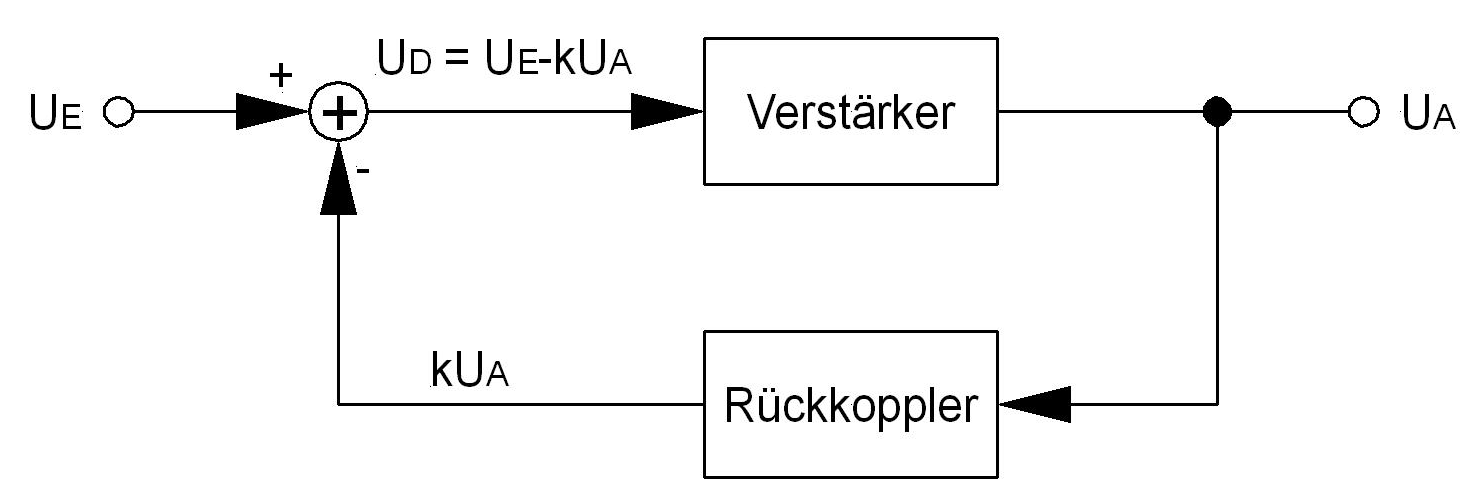
\includegraphics[width=1\textwidth]{a07/Gegenkopplung.png}
        \tiny \hyperlink{refs}{\cite{wm}} \\[3em]
     	\large
     \end{center}
    \begin{itemize}
			\item Für Mitkopplung muss Signal phasengleich sein
			\item Für Gegenkopplung muss Signal um $n \cdot 180$ verschoben sein
			\item Rückkopplung muss Verluste ausgleichen
			\item Zum Anschwingen Rückkopplung größer
    \end{itemize}
\end{frame}

\begin{frame}
    \frametitle{Meißner}
    \begin{center}
        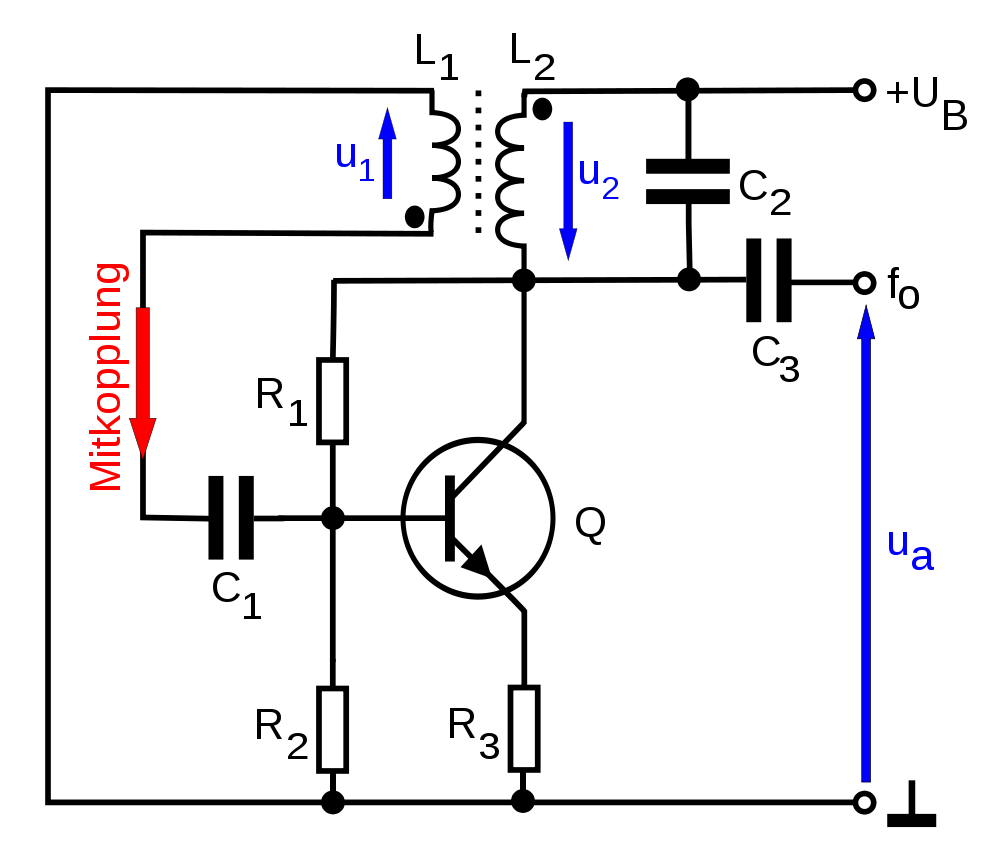
\includegraphics[width=0.67\textwidth]{a07/Meissner_oszi.png}
        \tiny \hyperlink{refs}{\cite{wm}} \\[1em] \large
     \begin{itemize}
			\item Benannt nach Alexander Meißner der 1913 Patentierte
			\item Rückkopplung über Transformator
			\item $180$ Transistor $+ 180$ Spule $= 360$ verschoben
    \end{itemize}
    \end{center}
\end{frame}

\begin{frame}
    \frametitle{Hartley}
    \begin{center}
        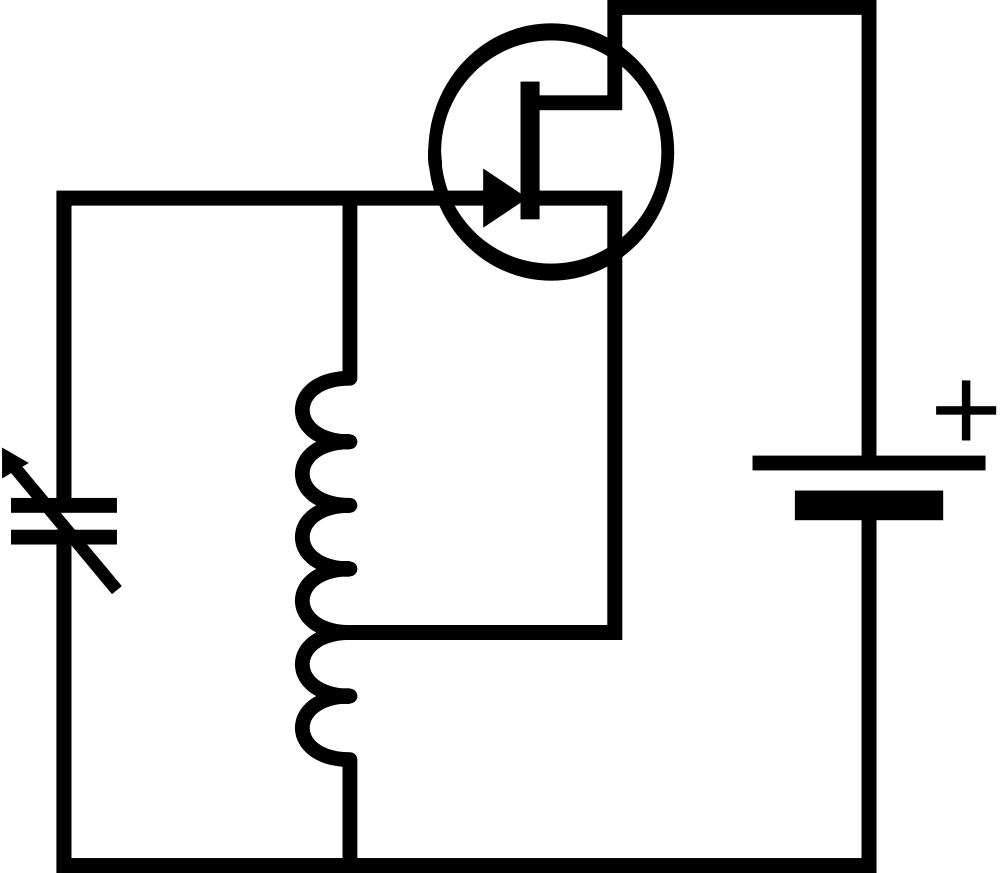
\includegraphics[width=0.67\textwidth]{a07/Hartley_osc.png}
        \tiny \hyperlink{refs}{\cite{wm}} \\[1em] \large
     	\begin{itemize}
			\item Benannt nach Ralph Hartley der 1920 Patentierte
			\item Rückkopplung über Spule die wie Trafo wirkt
			\item Spannung am Gate bewirkt Strom aus Source 
    	\end{itemize}
    \end{center}
\end{frame}

\begin{frame}
    \frametitle{Colpitts}
        \begin{center}
        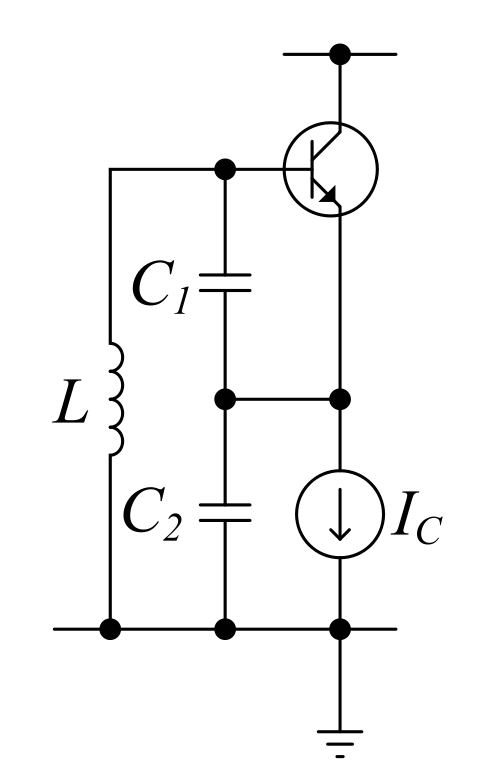
\includegraphics[width=0.4\textwidth]{a07/Cc_colp2.png} \\[1em] \large
     	\begin{itemize}
			\item Benannt nach Edwin H. Colpitts der 1918 Patentierte
			\item Rückkopplung über Kondensator
			\item Keine Phasenverschiebung da Kollektorschaltung
    	\end{itemize}
    \end{center}
\end{frame}

\begin{frame}
    \frametitle{Colpitts Beispiel}
        \begin{center}
        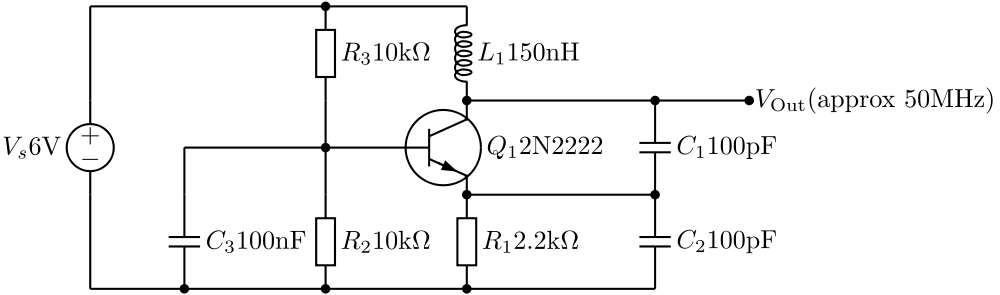
\includegraphics[width=1\textwidth]{a07/NPN_Colpitts_oscillator_collector_coil.png} \\[1em] \large
     	\begin{itemize}
			\item Hier Colpitts in Basisschaltung
    	\end{itemize}
    \end{center}
\end{frame}

\begin{frame}
    \frametitle{Zusammenfassung Dreipunkt-Schaltungen}
         \begin{itemize}
			\item Alle Oscillatoren möglich als Basis Kollektor oder Emitter
			\item Benannt nach Erfinder und unterschiedliche Rückkopplungen
			\item Colpitts sehr verbreitet da simple Spule
    	\end{itemize}
\end{frame}

\begin{frame}
    \frametitle{Quarzoszillator}
    \begin{center}
        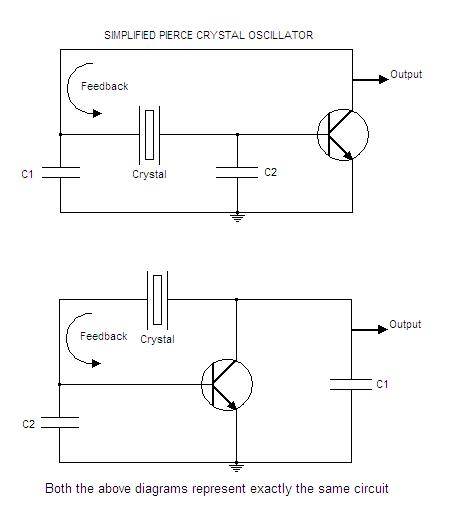
\includegraphics[width=0.62\textwidth]{a07/PIERCE_CRYSTAL_OSCILLATOR.jpg} \large
     	\begin{itemize}
			\item Quarzoszillator in Basis und Kollektorschaltung
    	\end{itemize}
    \end{center}
\end{frame}

\begin{frame}
    \frametitle{Quarzoszillator Besonderheiten}
    \large
         \begin{itemize}
			\item Sehr Frequenzstabiel
			\item Betrieb in Oberschwingung möglich mit Sperrkreis
			\item Oberschwingungen vielfaches der Grundfrequenz des Quarzes
    	\end{itemize}    
            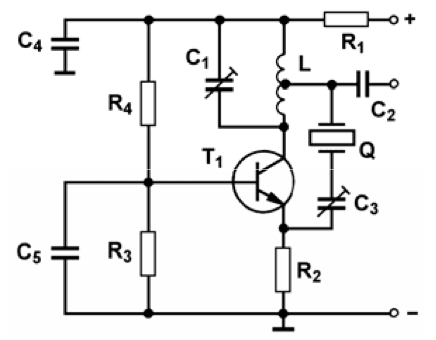
\includegraphics[width=0.7\textwidth]{a07/TD606_quarz_Oberschwingung.png}\\
            \tiny TD606 \hyperlink{refs}{\cite{bna}}
\end{frame}

\begin{frame}
    \frametitle{ }
            \begin{center}
         \Huge Pause
                 \end{center}
\end{frame}

\section*{Hf-Leistungsverstärker}

\begin{frame}
    \frametitle{Blockschaltbild Verstärkung}
    \begin{center}
        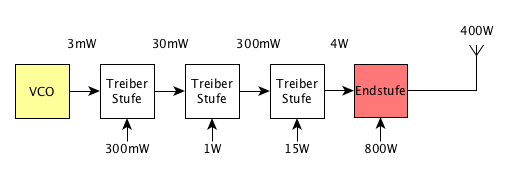
\includegraphics[width=1\textwidth]{a07/paBsb.png} \large
     	\begin{itemize}
			\item Verstärkung der Leistung in Stufen
			\item Meist höchstens $10dB$ verstärkung in den Treiberstufen
    	\end{itemize}
    \end{center}
\end{frame}

\begin{frame}
    \frametitle{Wirkungsgrad}
    \begin{center}
        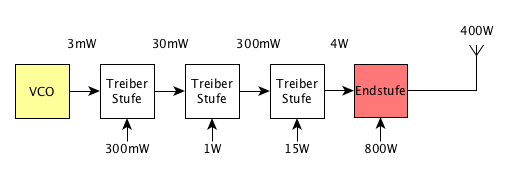
\includegraphics[width=1\textwidth]{a07/paBsb.png} \huge
     	\begin{itemize}
			\item Wirkungsgrad $\eta = \frac{P_{ausgang}}{P_{versorgung}}$
    	\end{itemize}
    \end{center}
\end{frame}

\begin{frame}
    \frametitle{Betriebsart Transistor}
    \begin{columns}[c]
        \column[c]{5cm}
        \begin{center}
            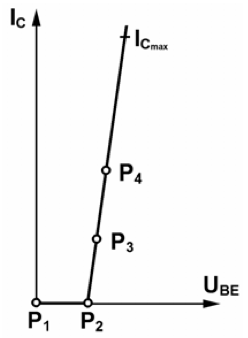
\includegraphics[width=1\textwidth]{a07/TD419.png}\\
            \tiny TD419 \hyperlink{refs}{\cite{bna}}
    \end{center}
    \column{5cm} \Large
	    \begin{enumerate} 
			\item $P_1$: C-Betrieb
			\item $P_2$: B-Betrieb
			\item $P_3$: AB-Betrieb
			\item $P_4$: A-Betrieb
    	\end{enumerate}
    \end{columns}
\end{frame}

\begin{frame}
    \frametitle{Betriebsart Röhre}
    \begin{center}
        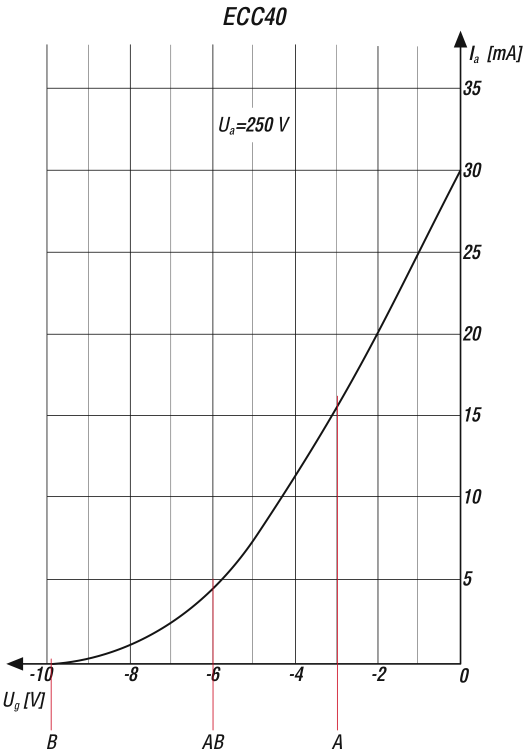
\includegraphics[width=0.54\textwidth]{a07/Ia_Ug_Kennlinie_ECC40.png} \\ \large
        Kennlinie mit Arbeitspunkten bei der Röhre ECC40
    \end{center}
\end{frame}

\begin{frame}
    \frametitle{Klasse-A}
        \begin{columns}[c]
        \column[c]{4cm}
        \begin{center}
            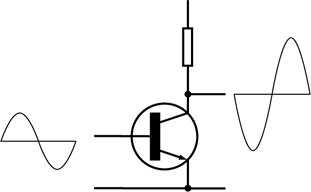
\includegraphics[width=1\textwidth]{a07/Electronic_Amplifier_Class_A.png}\\
            \tiny \hyperlink{refs}{\cite{wm}}
    \end{center}
    \column{5cm} \large
    \begin{block}{Klasse-A}
	    \begin{enumerate} 
			\item Beide Halbwellen werden verstärkt
			\item Hoher Verluststrom
			\item Kaum Signalverzerrung
			\item Einfacher Aufbau
			\item Um $40\%$ Wirkungsgrad
    	\end{enumerate}
    \end{block}
    \end{columns}
\end{frame}

\begin{frame}
    \frametitle{Klasse-B}
            \begin{columns}[c]
        \column[c]{4cm}
        \begin{center}
            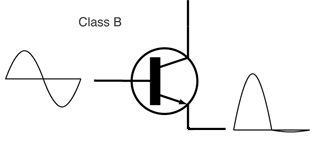
\includegraphics[width=1\textwidth]{a07/Electronic_Amplifier_Class_B_fixed.png}\\
            \tiny \hyperlink{refs}{\cite{wm}}
    \end{center}
    \column{5cm} \large
    \begin{block}{Klasse-B}
	    \begin{enumerate} 
			\item Nur die obere Halbwelle wird verstärkt
			\item Geringer Verluststrom
			\item Signalverzerrung
			\item Einfacher Aufbau
			\item Bis $80\%$ Wirkungsgrad
    	\end{enumerate}
    \end{block}
    \end{columns}
\end{frame}

\begin{frame}
    \frametitle{Klasse-AB}
        \begin{columns}[c]
        \column[c]{4cm}
        \begin{center}
            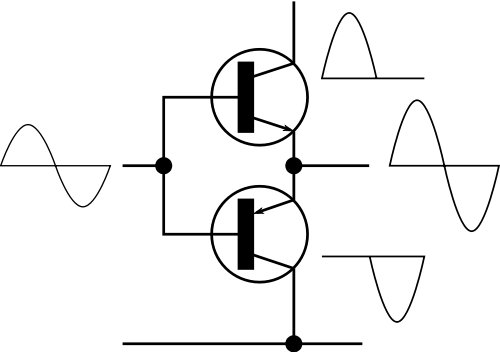
\includegraphics[width=1\textwidth]{a07/Electronic_Amplifier_Push-pull.png}\\
            \tiny \hyperlink{refs}{\cite{wm}}
    \end{center}
    \column{5cm} \large
    \begin{block}{Klasse-AB}
	    \begin{enumerate} 
			\item Ein Transistor pro Halbwelle
			\item Akzeptabler Verluststrom
			\item Minimale Signalverzerrung
			\item Komplizierter Aufbau
			\item Bis $75\%$ Wirkungsgrad
    	\end{enumerate}
    \end{block}
    \end{columns}
\end{frame}

\begin{frame}
    \frametitle{Klasse-C}
        \begin{columns}[c]
        \column[c]{4cm}
        \begin{center}
            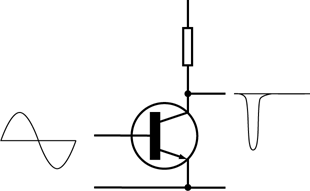
\includegraphics[width=1\textwidth]{a07/Electronic_Amplifier_Class_C.png}\\
            \tiny \hyperlink{refs}{\cite{wm}}
    \end{center}
    \column{5cm} \large
    \begin{block}{Klasse-C}
	    \begin{enumerate} 
			\item Nur Signalspitze wird verstärkt
			\item Quasi kein Verluststrom
			\item Starke Signalverzerrung
			\item Einfacher Aufbau
			\item Bis $87.5\%$ Wirkungsgrad
    	\end{enumerate}
    \end{block}
    \end{columns}
\end{frame}

\begin{frame}
    \frametitle{HF-Verstärkerschaltung}
    \begin{center}
        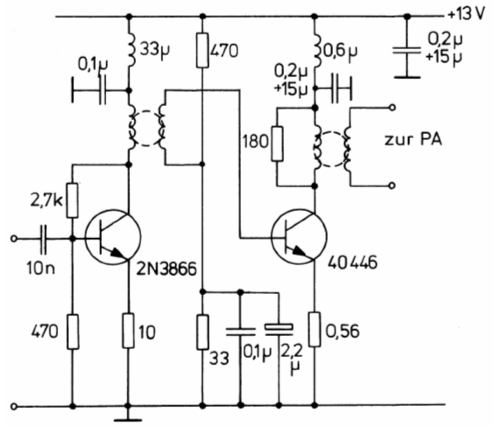
\includegraphics[width=0.85\textwidth]{a07/TG237.png}\\
        \tiny TG237 \hyperlink{refs}{\cite{bna}}
     	\begin{enumerate} \Large
			\item Breitband HF-Verstärker aus 2 Stufen
    	\end{enumerate}
    \end{center}
\end{frame}

\begin{frame}
    \frametitle{HF-Verstärkerschaltung Fragen}
        \begin{center}
        \begin{block}{TG238} \large
			 Ist die Schaltung um den 2N3866 eine Basis, Emitter oder Kollektor Schaltung?
    	\end{block}
        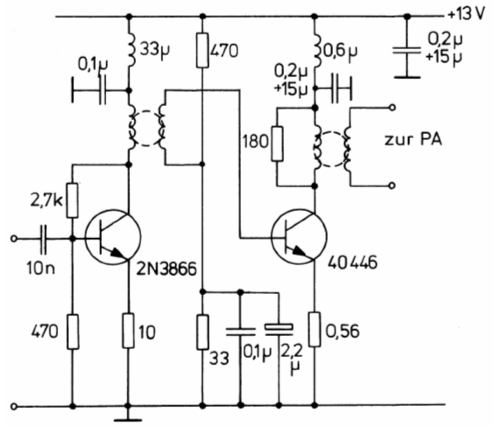
\includegraphics[width=0.7\textwidth]{a07/TG237.png}\\
        \tiny TG237 \hyperlink{refs}{\cite{bna}}
    \end{center}
\end{frame}

\begin{frame}
    \frametitle{HF-Verstärkerschaltung Fragen}
        \begin{center}
        \begin{block}{TG238} \large
			 Es handelt sich um eine Emitterschaltung.
    	\end{block}
        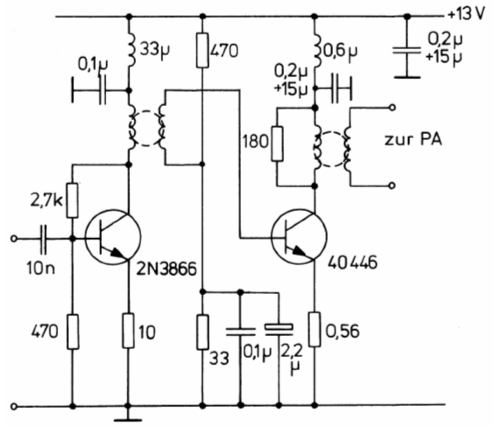
\includegraphics[width=0.7\textwidth]{a07/TG237.png}\\
        \tiny TG237 \hyperlink{refs}{\cite{bna}}
    \end{center}
\end{frame}

\begin{frame}
    \frametitle{HF-Verstärkerschaltung Fragen}
        \begin{center}
         \begin{block}{TG239} \large
			 Warum sind oft 2 C Parallel gegen Masse geschaltet?
    	\end{block}
        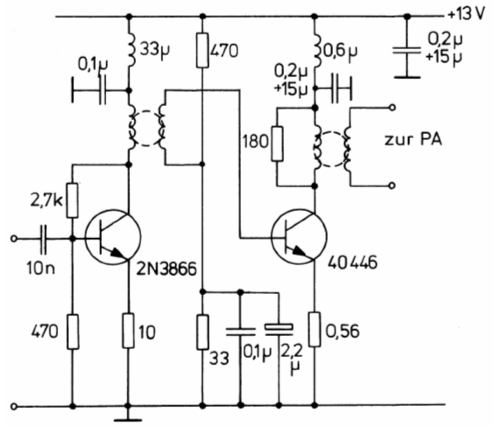
\includegraphics[width=0.7\textwidth]{a07/TG237.png}\\
        \tiny TG237 \hyperlink{refs}{\cite{bna}}
    \end{center}
\end{frame}

\begin{frame}
    \frametitle{HF-Verstärkerschaltung Fragen}
        \begin{center}
        \begin{block}{TG239}
		\large Der Kondensator mit der geringen Kapazität dient zur Siebung der hohen und der Kondensator mit der hohen Kapazität zur Siebung der niedrigen Frequenzen.
    	\end{block}
        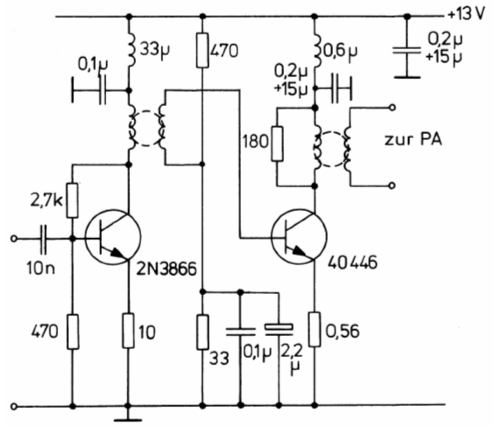
\includegraphics[width=0.65\textwidth]{a07/TG237.png}\\
        \tiny TG237 \hyperlink{refs}{\cite{bna}}
    \end{center}
\end{frame}

\begin{frame}
    \frametitle{FM-Verstärkerschaltung}
    \begin{center}
        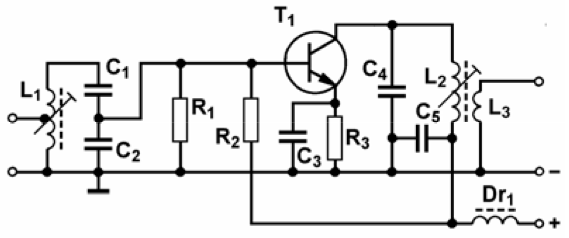
\includegraphics[width=1\textwidth]{a07/TG222.png}\\
        \tiny TG222 \hyperlink{refs}{\cite{bna}}
     	\begin{enumerate} \Large
			\item $2m$ FM-Endstufe
    	\end{enumerate}
    \end{center}
\end{frame}

\begin{frame}
    \frametitle{FM-Verstärkerschaltung Fragen}
    \begin{center} \Large
        \begin{block}{TG224}
		\large Welchem Zweck dient die Anzapfung an L1 in der folgenden Schaltung?
    	\end{block}
        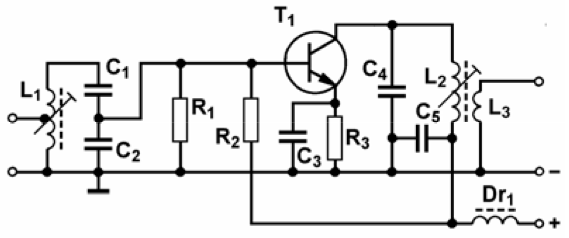
\includegraphics[width=1\textwidth]{a07/TG222.png}\\
        \tiny TG222 \hyperlink{refs}{\cite{bna}}
    \end{center}
\end{frame}

\begin{frame}
    \frametitle{FM-Verstärkerschaltung Fragen}
    \begin{center}\Large
        \begin{block}{TG224}
		\large Sie dient zur Anpassung der Eingangsimpedanz der Stufe.
    	\end{block}
        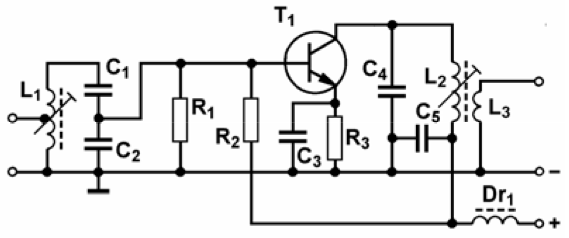
\includegraphics[width=1\textwidth]{a07/TG222.png}\\
        \tiny TG222 \hyperlink{refs}{\cite{bna}}
    \end{center}
\end{frame}

\begin{frame}
    \frametitle{FM-Verstärkerschaltung Fragen}
    \begin{center}\Large
        \begin{block}{TG225}
		\large Welchem Zweck dient C2 in der Schaltung?
    	\end{block}
        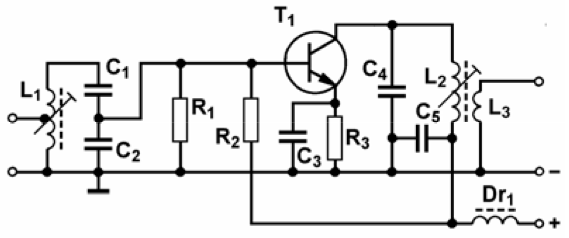
\includegraphics[width=1\textwidth]{a07/TG222.png}\\
        \tiny TG222 \hyperlink{refs}{\cite{bna}}
    \end{center}
\end{frame}

\begin{frame}
    \frametitle{FM-Verstärkerschaltung Fragen}
    \begin{center} \Large
        \begin{block}{TG225}
		\large Zur Festlegung der HF-Kopplung \\
		Merke: Bei Fragen mit Kondensatoren immer die HF-Antwort
    	\end{block}
        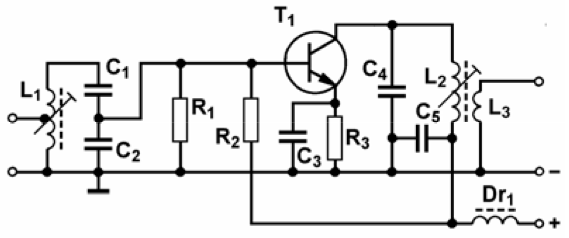
\includegraphics[width=1\textwidth]{a07/TG222.png}\\
        \tiny TG222 \hyperlink{refs}{\cite{bna}}
    \end{center}
\end{frame}

\begin{frame}
    \frametitle{HF-Verstärker mit Röhren}
    \begin{center}
        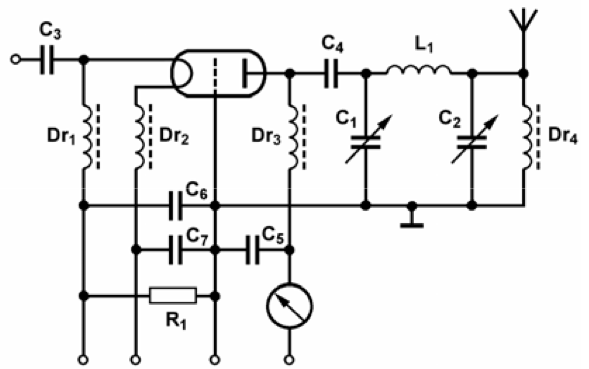
\includegraphics[width=1\textwidth]{a07/TG313.png}\\
        \tiny TG313 \hyperlink{refs}{\cite{bna}}
     	\begin{enumerate} \Large
			\item Röhrenendstufe mit Pi-Filter am Ausgang
    	\end{enumerate}
    \end{center}
\end{frame}

\begin{frame}
    \frametitle{Röhrenverstärker abstimmen}
    \begin{center} \Large
        \begin{block}{TG315}
		\large An dem Drehknopf für $C_1$ steh $C_{Plate}$ oder "Plate", an dem für $C_2$ steht $C_{Load}$ oder "Load". Die drei Bauelemente $C_1$, $C_2$ und $L_1$ bilden zusammen einen so genannten Pi-Tankkreis zur Anpassung der Ausgangsimpedanz der Röhre an die Antennenimpedanz.\\
    	\end{block}
        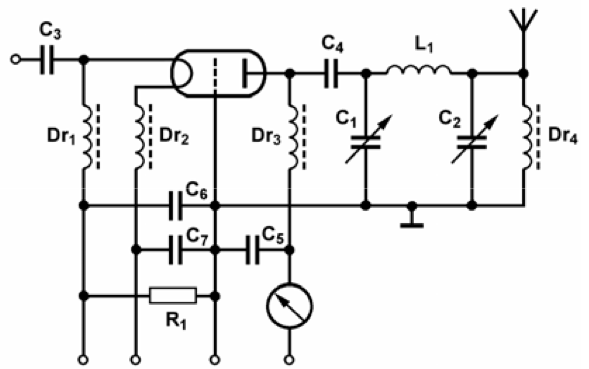
\includegraphics[width=0.65\textwidth]{a07/TG313.png}\\
        \tiny TG222 \hyperlink{refs}{\cite{bna}}
    \end{center}
\end{frame}

\begin{frame}
    \frametitle{Röhrenverstärker abstimmen}
    \begin{center} \Large
        \begin{block}{TG316}
		\large
		Zum Abstimmen $C_1$ und $C_2$ auf maximale Kapazität stellen. $C_1$ auf Dip im Anodenstrom (Resonanz) stellen, dann mit $C_2$ einen etwas höheren Anodenstrom einstellen (Leistung auskoppeln). Vorgang mit $C_1$ und $C_2$ wechselweise mehrmals wiederholen bis die maximale Ausgangsleistung erreicht ist.
    	\end{block}
        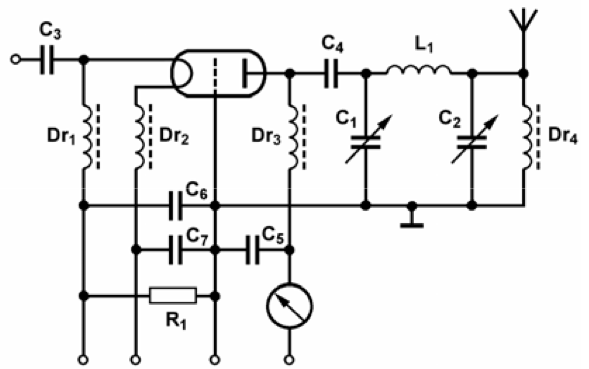
\includegraphics[width=0.6\textwidth]{a07/TG313.png}\\
        \tiny TG222 \hyperlink{refs}{\cite{bna}}
    \end{center}
\end{frame}

\section*{Leistungsangaben}

\begin{frame}
    \frametitle{Senderleistung}
        \begin{block}{TG901} \Large
			Die Sendeleistung eines Senders ist  die unmittelbar nach dem Senderausgang messbare Leistung, bevor sie Zusatzgeräte (z.B. Anpassgeräte) durchläuft. \\
			Angegeben als PEP bei SSB oder Trägerleistung bei FM AM CW
	    \end{block}
\end{frame}

\begin{frame}
    \frametitle{Spitzenleistung}
        \begin{block}{Spitzenleistung (engl. peak envelope power, PEP)} \Large
			PEP bezeichnet die mittlere hochfrequente Leistung am Ausgang einer Sendeendstufe, während das modulierende Signal seinen Spitzenwert hat.\\
			Wird meist bei SSB angegeben.
	    \end{block}
\end{frame}

\begin{frame}
    \frametitle{Strahlungsleistung}
        \begin{block}{ERP} \Large
			Leistung aus der Antenne im Vergleich zu Dipol
	    \end{block}
        \begin{block}{EIRP} \Large
			Leistung aus der Antenne im Vergleich zu Isotropher Kugelstrahler
	    \end{block}
\end{frame}

\begin{frame}
    \frametitle{Mittlere Leistung}
        \begin{block}{Mittlere Leistung} \Large
			Durchschnittliche Leistung, die ein Sender unter normalen Betriebsbedingungen während eines Zeitintervalls als HF-Leistung abgibt.
	    \end{block}
\end{frame}

\begin{frame}
    \frametitle{Signalverzerrung}
        \begin{center}
        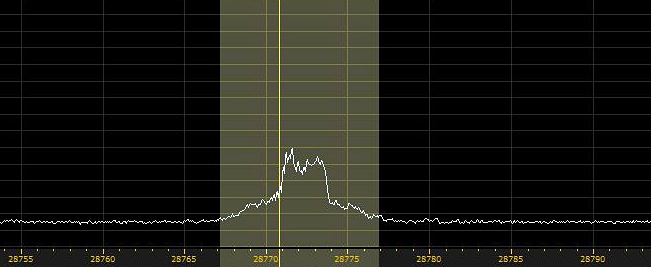
\includegraphics[width=1\textwidth]{a07/splatter.jpg}\\[1em]
     	\large Zu starke Verstärkung führz zu Unlinearer Verstärkung, also Verzerrung des Signals und Splatter\\
     	$10dB$ pro Decade. Normales SSB-Signal $3kHz$, dieses $9kHz$
     \end{center}
\end{frame}

\renewcommand{\refname}{Referenzen}

\hypertarget{refs}{}
\textcolor{white}{} \\ %\vspace{} geht nicht
\Large Referenzen/Links
\footnotesize

\begin{thebibliography}{}
    \bibitem{darc}  DARC Online-Lehrgang Lektion A07:
                    \url{http://www.darc.de/referate/ajw/ausbildung/darc-online-lehrgang/technik-klasse-a/technik-a07/}
    \bibitem{wm} 	Wikimedia:
                    \url{https://commons.wikimedia.org/wiki/File:Closed_loop_gain.png}
                    \url{http://commons.wikimedia.org/wiki/File:HF-Ersatzschaltbild.svg}
                    \url{https://commons.wikimedia.org/wiki/File:Lawine.jpg}
                    \url{https://commons.wikimedia.org/wiki/File:Gegenkopplung.png}
                    \url{https://commons.wikimedia.org/wiki/File:Meissner_oszi.svg}
                    \url{https://commons.wikimedia.org/wiki/File:Hartley_osc.svg}
                    \url{https://commons.wikimedia.org/wiki/File:NPN_Colpitts_oscillator_collector_coil.svg}
                    \url{https://commons.wikimedia.org/wiki/File:PIERCE_CRYSTAL_OSCILLATOR.jpg}
                    \url{https://commons.wikimedia.org/wiki/File:Electronic_Amplifier_Class_A.png}
                    \url{https://en.wikipedia.org/wiki/File:Electronic_Amplifier_Class_B_fixed.png}
                    \url{https://commons.wikimedia.org/wiki/File:Electronic_Amplifier_Push-pull.svg}
                    \url{https://en.wikipedia.org/wiki/File:Electronic_Amplifier_Class_C.png}
                    \url{}
                    \url{}
                    \url{}
                    \url{}
    \bibitem{wp}    Wikipedia - Die freie Enzyklopädie:
                    \url{https://de.wikipedia.org/wiki/Gleichrichter}
	\bibitem{bna}   Fragenkatalog Bundesnetzargentur Technik Klasse A:                   
                    \url{https://www.bundesnetzagentur.de/SharedDocs/Downloads/DE/Sachgebiete/Telekommunikation/Unternehmen_Institutionen/Frequenzen/Amateurfunk/Fragenkatalog/TechnikFragenkatalogKlasseAf252rId9014pdf.pdf?__blob=publicationFile&v=3}
    \bibitem{fi}    Freie Inhalte (DK0TU):
                    \url{http://www.dk0tu.de/Projekte/Freie_Inhalte/}
\end{thebibliography} 

% Hier könnte noch eine Kontaktfolie stehen

\end{document}

